\documentclass[26pt,fleqn,]{report}
%\usepackage[]{amsmath}
\usepackage[]{mathtools}
\usepackage[utf8]{inputenc}
\usepackage[T1]{fontenc}
\usepackage{lmodern}
\usepackage{xytree}
\usepackage{enumitem}
\usepackage{graphicx}
\DeclareGraphicsExtensions{.pdf,.png,.jpg}
\date{}

\begin {document}
%\large
\title{{\huge Graduation Research 3 Report}\\
Linguistic Logic Reasoning:\\
Implementation of Alpha Resolution on fuzzy propositional logic based on Linear Symmetrical Hedge algebra\\
}
\author{Instructor: Tran Dinh Khang\\Student: Ngo Nhat Anh, ID: 20090102}
\maketitle

%test
%\begin{align}
%e^i\pi\\ A \in B \\B \ni A \\A \not\ni B \\M > N \\\bar{A} \equiv B \cap \bar{C}
%\end{align}
%endtest
%
%

\chapter{Theoretical Background}


\section{Hedge algebra}
\subsection{Definition}
{\bfseries Linguistic hedge:} a unary operation on linguistic value, changing the linguistic value's meaning.
\\
{\bfseries Hedge algebra:} Let \(X\) be a linguistic variable and its domain is \(X = Dom(X)\). A hedge 
algebra \(AX\) in respect to \(X\) is a 4-tuple \(AX = (X,G,H,\le)\) where G is the set of spanning
elements, H is the set of hedges and \(\le\) is the sematic ordering relation on X.
The set G usually has positive, negative and neutral spanning elements. In practice, G usually has only
positive and negative spanning elements e.g \{True,False\}, \{High, Low\}.\\

A hedge algebra AX satisfies the following  axioms:\\
{\indent
	(1) Hedges either increase or decrease the effect of other hedges including itself, and it is 
then positive or negative w.r.t. the other.\\}
{\indent
	(2) If \(u\notin H(v)\) and \(v\notin H(u)\) then \(\forall x\in H(u), x\notin H(v)\) and vice versa. 
	Furthermore if u and v cannot be compared then so are x,y for all \(x\in H(u), y\in H(v)\).
}\\
{\indent
	(3) \(x \not = hx, x \notin H(hx). h\neq k, hx<kx\) then \(h'hx\le k'kx\forall h,h',k,k'\in
	H.\) Furthermore, if \(hx \neq kx\) then hx and kx are independent w.r.t. to each other.
}\\
{\indent
	(4) \(u \in v, u \le v\implies u\le hv\) for \(\forall h\) and vice versa.
}
\\\\
(1) means exactly what it says.\\
(2) means that if two vague concepts are really different, then they form seperated concept categories,
which means they don't have any common meaning.\\
(3) means that each hedge has its own meaning and defines its own concept category.\\
(4) means that a hedge only modifies the vague concept's meaning. It preserves the ordering relation
of the vague concept's meaning w.r.t. other vague concepts.\\
\subsection{Properties}
	{\bfseries Semantic heredity:} When a hedge affects the meaning of a linguistic value, it only
	increases or decreases a little bit the meaning of that value. The resulting value inherits
	most of its parent's meaning i.e the parent's comparability is preserved: 
	if hx \(\le\) kx then H(hx) \(\le\) H(kx). Generally, \(\forall (u,v \in X, 
	\sigma_1 = h_n..h_1, \sigma_2 = k_m..k_1, h_i,k_j \in H)\), we have:
	\(u \le v \implies \sigma_1u \le \sigma_2v\)\\
	{\bfseries Theorem 1:} Let AX = (X,G,H,\(\le\)). The following statements hold:\\
\indent (1) If x \(\in\) X is a fixed point of an operation h in H, i.e. hx = x, then it is a fixed
	 point of the others.\\
\indent (2) If x = \(h_n \cdots h_1 u\), and there exists an index \(i<n\) such that \(h_i \cdots h_1 u\)        is another representation (canonical) of x w.r.t. u and \(h_j x = x, \forall j\ge i\).\\
\indent (3) For any \(h, k\in H\), if \(hx\le kx\) and \(h\neq k\) then \(hx< kx\).\\
\indent \(\implies\) The canonical representation of any linguistic value w.r.t. another value is unique.	\\
\indent {\bfseries Theorem 2:} Let \(x = h_n \cdots h_1 u\) and \(y = k_m \cdots k_1 u\) be two arbitrary
	canonical representations of x and y w.r.t. u, respectively. Then there exists an index
	\(j \le min{n, m} + 1\) such that \(h_i = k_i, \forall i < j\), and\\
\indent (1) \(x < y \iff h_j x_j < k_j x_j , where x_j = h_j-1 \cdots h_1 u\)\\
\indent (2) \(x = y \iff n = m = j and h_j x_j = k_j x_j\)\\
\indent (3) x and y are incomparable \(\iff h_j x_j\) and \(k_j x_j\) are incomparable\\
\indent \(\implies\) This theorem provides us the mean to compare two linguistic value in a hedge 
algebra. 

\subsection{Linear symmetrical algebra}
The spanning set G usually has two comparable linguistic values. For example, we have False \(<\) True
for truth value. A hedge algebra that has only two primitive linguistic values is called a symmetrical
hedge algebra. The spanning set is denoted \(G = \{c^-, c^+\}, c^+, c^-\) are positive and negative 
spanning element, respectively.\\\\

The set H of hedges can also be partitioned into two seperated subsets \(H^+ = \{h|hc^+ > c^+\} = 
\{h|hc^- < c^-\}, H^- = \{h|hc^- > c^-\} = 
\{h|hc^+ < c^+\}\). Any two hedges in \(H^+\) (or \(H^-\)) are comparable to each other, and each hedge in \(H^+\) is converse to a hedge in \(H^-\) and vice versa. A hedge algebra \(AX = (X,\{c^+,c^-\},H^+\cup
H^-, \le)\) is linear symmetrical iff \(H^+\) and \(H^-\) are linearly ordered. It is easy to see
that X is also linearly ordered by \(\le\).\\\\

Let I \(\notin\) H be the {\em identity hedge}: \(\forall x \in X, Ix = x\). I is smaller than any other
hedge in \(H^+\) and \(H^-\).\\\\

If \(H \neq {\o}, H(c^+), H(c^=)\) are infinite then \(inf(c^+) = sup(c^-) = W, inf(c^-) = 0, sup(c^+) = 1\). W is call the neutral element. We have: \(0<c^-<W<c^+<1\). Denote the linguistic value domain as
\(\bar X = X \cup \{0,W,1\}\)\\\\

From that we define:
\begin{itemize}
\item Let \(x = \sigma c, \sigma \in H^*, c \in \{c^+, c^-\}. y \text{is the negation of x, denoted}
	y = -x \text{ if } y = \sigma c', \{c,c'\} = \{c^+, c^-\}. -0 = 1, -1 = 0, -W = W\).
\item \(x,y \in \bar X\) then \(x \wedge y = min(x,y), x \vee y = max(x,y)\)
\end{itemize}


\subsection{Rule of moving hedges}
\indent (RT1): \(\frac{((P,hu),\sigma <True|False>)} {((P,u),\sigma h<True|False>)}\)
\\
\\
	(RT2): \(\frac{((P,u),\sigma h<True|False>)} {((P,hu),\sigma <True|False>)}\)
\section{A propositional logic with truth value domain based on LSA}
\subsection{Syntax}
\indent {\bfseries The alphabet of logic} consists of the following classes of symbol:\\
\indent + Propositional symbols: A,B,C \ldots\\
\indent + Linguistic value symbols: a,b,c \ldots\\
\indent + Constant symbols: 0,1,W\ldots\\
\indent + Logical connectives:\(\vee,\wedge,\to,\neg\) \ldots\\
\indent + Auxiliary symbols: ',', '(', ')'\ldots\\ \\
{\bfseries Literal:} A string \(A^a\), where \(A\) is a propositional symbol and \(a\) is a truth
value in \(A\)'s domain.\\\\
 {\bfseries Formula:}\\
 \indent + A literal is a formula\\
 \indent + F is a formula then \( (\neg F\)) is also a formula\\
 \indent + F and G are formulae then \( (F\vee G), (F\wedge G), (F \to G)\) are also formulae\\
 \indent + Only strings generated by the above rules are formulae\\
 \indent ( {\bfseries Precedence of operations:} \(\neg\)  >>  \(\to\)  >>  \(\wedge\)  >>  \(\vee\))\\

\subsection{Semantic}
\subsubsection{Interpretation}
An {\bfseries Interpretation} I:\{A = a1\} of the literal \(A^{a2}\) is the mapping associate the formula
with a value of the truth value domain.\\

{\bfseries Logical connectives' semantics:} let a and b be some linguistic value. Then:\\
\indent + \(a \vee b = max(a,b)\)\\
\indent + \(a \wedge b = min(a,b)\)\\
\indent + \(\neg a = \text{symmetrical value of } a\)\\
\indent + \(a \to b = max(\neg a,b)\)\\
\(\implies \wedge\) and \(\vee\) are G{\"o}del's T-norm and T-conorm.\\
Let T(A) be A's truth value under an arbitrary interpretation.\\
{\bfseries Truth value of formulae:}\\
\indent + If A is a literal, T(A) is determined by the interpretation\\
\indent + Let A and B be two formulae:\\
\indent \indent (1) \(T(A\vee B) = T(A) \vee T(B)\)\\
\indent \indent (2) \(T(A\wedge B) = T(A) \wedge T(B)\)\\
\indent \indent (3) \(T(A\to B) = T(A) \to T(B)\)\\
\indent \indent (4) \(T(A\neg B) = T(A) \neg T(B)\)
\\\\
Let \(T_{I:\{A = a1\}}(A^{a2})\) the value of that interpretation. Then:\\
\indent + \(T_{I:\{A = a1\}}(A^{a2}) = a1 \wedge a2 \) if a1, a2 \(\ge W\)\\
\indent + \(T_{I:\{A = a1\}}(A^{a2}) = \neg (a1 \vee a2) \) if a1, a2 \(<\) W\\
\indent + \(T_{I:\{A = a1\}}(A^{a2}) = \neg a1 \vee a2 \) if a1 \(\ge\) W, a2 \(<\) W\\
\indent + \(T_{I:\{A = a1\}}(A^{a2}) =  a1 \vee \neg a2 \) if a1 \(<\) W, a2 \(\ge\) W\\

\subsubsection{Satisfiable, unsatisfiable, false}
{\bfseries Definition:} Let S be a formula, I be an arbitrary interpretation:\\
\indent + S is false under I if \(T_I(S) < W\)\\
\indent + S is unsatisfiable if it is contradicted to every interpretation\\ 
\indent + S is satisfiable if \(\exists I: T_I(S) \ge W\). I is then called a model of S, denoted \(I \models S\)\\
\indent + S is a tautology if \(\forall I: T_I(S) \ge W\)\\
\indent \(\implies)\) Collorary: A formula A is a tautology iff \(\neg\)A is unsatisfiable.
\subsubsection{Logical equivalences. Functional complete set of logical connectives}
\indent Two formula A abd V are said to be equivalent (\(A \equiv B\)) if A and B have the same \\
indent truth value for every interpretation I.\\
\indent Some well-known logical equivalences:
\begin{align*}
+ A \to B \equiv \neg A \vee B\\
+ A \to B \equiv \neg A \vee B\\
+ A \to B \equiv \neg A \vee B\\
+ A \to B \equiv \neg A \vee B\\
+ A \to B \equiv \neg A \vee B\\
+ A \to B \equiv \neg A \vee B\\
+ A \to B \equiv \neg A \vee B\\
+ A \to B \equiv \neg A \vee B\\
+ A \to B \equiv \neg A \vee B\\
\end{align*}
\indent {\bfseries Functionally complete set of logical connectives} is one which can be used to express all possible logical functions \(f:TV^n \to TV\)\\
\subsubsection{Conjunctive normal form}
A formula expressed as a conjunction of formulae, where these formulae are in turn expressed as
a disjunction of literal, is said to be in {\em Conjunctive normal form}.\\
{\bfseries Theorem:} Every formula in our propositional logic is logically equivalent to a CNF
formula.\\
Algorithm to transform a formula into its CNF:\\\\
\indent- Eliminate \(\to\) and \(\leftrightarrow\) :
\begin{align*}
	&F \to G \underset{CNF}{\implies} \neg F \vee G\\
	&F \leftrightarrow G \underset{CNF}{\implies} (\neg F \vee G) \wedge (\neg G \vee F)
\end{align*}
\indent- Move \(\neg\) inward: 
\begin{align*}
	&\neg (F \vee G) \underset{CNF}{\implies} \neg F \wedge \neg G
\end{align*}
\indent- Elimitate double negation:
\begin{align*}
	&\neg \neg F \underset{CNF}{\implies} F
\end{align*}
\indent- Applying distributivity law:
\begin{align*}
	&F \wedge (G \vee H) \underset{CNF}{\implies} (F \wedge G) \vee (F \wedge H)\\
	&F \vee (G \wedge H) \underset{CNF}{\implies} (F \vee G) \wedge (F \vee H)
\end{align*}	
\indent- Rewrite redundant formula:
\begin{align*}	
	&F \vee F \underset{CNF}{\implies} F\\
	&F \wedge F \underset{CNF}{\implies} F
\end{align*}
\subsection{Inference}
\subsubsection{Logical consequence}
{\bfseries Logical consequence:} A is a logical consequence of B if every interpretation 
satisfying A also satisties B. Notated: A \(\models\) B.\\
\subsubsection{Inference rule:}
{\bfseries Inference rule:} An inference rule of the form\\
\begin{align*}
	\frac{F_1, F_2,\cdots,F_n}{G}
\end{align*}
means that with a given set of formula \(F_1,F_2,\cdots,F_n\), we can deduce a 
new formula \(G\). An inference rule is sound if it satisfies logical consequence.\\\\
To be useful, aside from being sound, an inference rule also should be complete, meaning\\
it deduce every formula that is a logical consequence of the original set of formulae.\\

%
%
\section{Resolution in HA-based logic}
\subsection{Resolution rule}
{\bfseries Resolution rule:} Given \(A^a \vee B^{b1}\) and \(C^c \vee B^{b2}\). If \(b1 \vee b2 
\ge W\) and \(b1 \wedge b2 < W\):
\begin{align*}
	&\frac{(A^a \vee B^{b1}, {\alpha 1}), (C^c \vee B^{b2}, {\alpha 2})} {(A^a \vee C^c, {\alpha 3})}\\
	&\text{Where: }
	\begin{cases}
	\alpha 1, \alpha 2, \alpha 3 \text{ are the reliability of formulae.}\\
	A, B, C \text{ are propositional symbols}\\
	a, b1, b2, c \text{ are linguistic value}
	\end{cases}
	\\
	&\text{If } (A^a \vee B^{b1}, {\alpha 1}) \wedge (C^c \vee B^{b2}, {\alpha 2}) \text{ is 
	unsatisfiable, the result of resolution is the null clause.} 
\end{align*}
\(\implies\) To be able to reasoning using resolution, we first have to transform the original
formulae into their CNFs.\\


{\bfseries Resolution algorithm:} 
 To prove that a goal clause G entails the knowledge base KB, e.g \(KB \models G\), we can instead prove
that \(KB \cup \neg G\) is unsatisfiable.\\\\
\indent {\em Input: S = \(KB \cup \neg G\)}\\
\indent {\em Output: S is unsatisfiable or not}\\\\
\indent{\bfseries BEGIN}\\
\indent If (S contains NULL) thenn return true;\\
\indent Foreach (clause C1 in S)\\
\indent \indent Foreach (clause C2 in S)\\
\indent \indent \indent If (C1 and C2 can be resolved) C3 := resolve(C1,C2);\\
\indent \indent \indent If (C3 = NULL) return true;\\
\indent \indent \indent Else (Add C3 to S);\\
\indent If (S does not contain NULL) then return false;\\
\indent{\bfseries END}\\


\subsection{Reliability value in HA-based logic}
By the definition of resolution, we can see for the two clauses to be able to resolve, \(b_1\) and 
\(b_2\) must be on different side w.r.t. W, and the bigger their difference, the more reliable the 
inference.\\\\
The reliability \({\alpha}_3\) of the inferred clause is:\\
\begin{align*}
	{\alpha}_3 = \wedge({\alpha}_1, {\alpha}_2, (b_1 \vee b_2), \neg(b_1 \wedge b_2))
\end{align*}
\\
\subsection{Alpha-resolution stragety in HA-based logic}
\paragraph{} Since different proofs of the same clause may have different reliabilities, 
it is natural to study how to design a resolution procedure with the best reliability. 
Below we present such a procedure.
\paragraph{} 
We say that a set of clauses S is saturated iff for every fuzzy linguistic reso-
lution inference with premises in S, the conclusion of this inference is a variant
with smaller or equal reliability of some clauses in S. That is for every fuzzy
linguistic resolution inference:\\
\[\indent \frac{(C1, \alpha1), (C2, \alpha2)}{(C,\alpha)}
\]
\indent there is some clause \((C',\alpha') \in \) S such that \(\alpha' \ge \alpha\).
\paragraph{} 
We introduce a resolution strategy, called $\alpha$-strategy, which guarantees that
the resolution proof of each clause has the maximal reliability. An $\alpha$-strategy
derivation is a sequence of the form $S_{0},\ldots,S_{i},\ldots$, where
\begin{itemize} 
	\item each Si is a set of clauses with reliability, and
	\item  \(S_{i+1}\) is obtained by adding the conclusion of a fuzzy 
	linguistic resolution inference with premises with maximal reliabilities 
	from Si , that is \(S_{i+1} = Si \cup \{(C, \alpha)\}\), 
	where (C, $\alpha$) is the conclusion of the fuzzy linguistic resolution inference  
	\(\frac{(C1 , \alpha1), (C2 , \alpha2)}	{(C, \alpha)}\)
	\\\\	
	$(C1 , \alpha1 ), (C2 , \alpha2 ) \in S_{i}$ and there are not any clauses 
	with reliability $(C1 , \alpha_{1}' ), (C2 , \alpha_{2}' ) \in S_{i}$ such that
			$\alpha_{1}' > \alpha_{1}$ and $\alpha_{2}' > \alpha_{2}$ , or

		\item $S_{i+1}$ is obtained by removing a variant with smaller 
			reliability, that is $S_{i+1} = S_{i} \setminus \{(C, \alpha)\}$ 
			where $(C, \alpha) \in S_{i}$ and there is some
			$(C, \alpha') \in S_{i}$ such that $\alpha < \alpha'$.
\end{itemize}
\paragraph{} 
{\bfseries The limit of a derivation $S_{0},\ldots,S_{i},\ldots$:} 
$S_{\infty} = \underset{i \ge 0}{\cup} \underset{j \ge i}{\cap}S_{j}$
\\
The following result establishes the soundness and completeness of the reso-
lution procedure.
\paragraph{Theorem 2}
Let $S_{0},\ldots,S_{i},\ldots$ be a fuzzy linguistic resolution $\alpha$-strategy derivation.
Sn contains the empty clause iff S0 is unsatisfiable (for some n = 0, 1,\ldots).
\paragraph{Lemma 2} 
Consider the following resolution inferences:
\[ \frac{(A^{a} \vee B^{b1}, \alpha), (B^{b2} \vee C^{c}, \beta)} {(A^{a} \vee C^{c}, \gamma)}\]
\[\frac{(A^{a} \vee B^{b1}, \alpha), (B^{b2} \vee C^{c}, \beta')} {(A^{a} \vee C^{c}, \gamma')}\]
Then, $\beta' > \beta$ implies $\gamma' \ge \gamma$

\paragraph{Lemma 3} Let $S_{0},\ldots,S_{i},\ldots$ be a fuzzy linguistic 
resolution $\alpha$-strategy derivation, and $S_{\infty}$ be the the limit of the derivation.
Then $S_{\infty}$ is saturated.

\paragraph{Theorem 3} Let $S_{0},\ldots,S_{i},\ldots$ be a fuzzy linguistic 
resolution $\alpha$-strategy derivation, and $S_{\infty}$ be the the limit of the derivation. 
Then for each clause $(C, \alpha)$ in $S_{\infty}$ , there is not any other resolution proof 
of the clause $(C, \alpha')$ from $S_{0}$ such that $\alpha' > \alpha$.


\chapter{System Design}

\section{Overview}
	
\paragraph{} The main objective of this project is to demonstrate the applicability and feasibility of automated linguistic logic reasoning systems based on linear symmetrical hedge algebralso intenda, to design and implement a system for developing knowledge bases capable of capturing fuzzy linguistic 
concepts, as an alternative to traditional fuzzy logic knowledge base, and as an optional goal, to later extend it into a fuzzy hedge algebra based logic programming system.\\

\paragraph{} The system in this report is a reasoning system using a propositional logic with user-defined linear symmetrical hedge algebra as the domain of truth value. The reasoning method to be used is the aforementioned Alpha Resolution in the previous part.

\subsection{Problem Definition}

\paragraph{}Essentially, the general problem to be solved by this system is, given a linear symmetrical hedge algebra (LSHA) as a truth value domain, a set of hedge algebra based propositional CNF clauses and a goal clause, show how “true” that clause is.\\

\paragraph{}The initial input of the program is a database describing the hedge algebra to be used, and another database where the knowledge base is stored.\\
The hedge database including:

\begin{itemize}
\item A table defining the hedges of the LSHA, including the hedges, their id, the negativity/positivity of the hedge.
\item Two tables for the positive/negative hedges, and their ordering.
\item A table defining the positive/negative relationship matrices between hedges.
\end{itemize}

\paragraph{}The generator terms of the hedge algebras are always Tru and Fals, so they don't need to be specified. There are also two other constant: MaxT for the maximum truth value, and MinT for the minimum truth value, regardless of the set of hedges.\\

\paragraph{}The knowledge base database including:

\begin{itemize}
\item A table describing CNF clauses, including their id and their clause string. 
\end{itemize}

\paragraph{} The rest of the input are user's interactions with the system.
\paragraph{} The Output is a linguistic truth value for the queried clause, or Nothing if it was unprovable. If the user chose to write the modified knowledge base, then that would also be an output of the system.


\subsection{Technologies used}

\paragraph{}The programming language being used is Haskell, a purely functional programming language. The reason behind this choice is the language's powerful type system that naturally suits for describing mathematical constructs such as hedge algebras, and its enforcement of functional programming style, whose expressiveness can enable the design of very modular and even composable programs. The particular implementation of Haskell used for this system is the Glasgow  Haskell Compiler v.7.4.2 on Linux.

\paragraph{}The chosen database management system is the lightweight embedded DMBS SQLite3. 

\paragraph{}The system required three Haskell libraries: 

\begin{itemize}
\item Parsec, a parser combinators library is chosen for implementing the the clause strings parser
\item HDBC, the Haskell Database Connectivity library
\item HDBC.SQLite3, SQLite3's backend for HDBC
\end{itemize}

\section{High level Requirements}
\subsection{Functional Requirements}
\begin{itemize}
\item Allow user defined hedge algebra
\item Allow user to load, edit, print and write knowledge base 
\item Allow user to prove any valid clause
\end{itemize}

\subsection{Non- Functional Requirements}
\begin{itemize}
\item Acceptable performance
\item Easy to use
\end{itemize}

\subsection{Quality Attributes}

\paragraph{Correctness:}
Automated reasoning method must be sound and refutation-complete

\paragraph{Maintainability:}
The system should be easy to maintain and extend
\section{Data description}


\subsection{Overview}

\paragraph{}There are two databases: one for describing the hedge algebra to be used, and another for storing the knowledge base.\\

\paragraph{}The hedge database including:

\begin{itemize}
\item A table defining the hedges of the LSHA, including the hedges, their id, the negativity/positivity of the hedge.
\item Two tables for the positive/negative hedges, and their ordering.
\item A table defining the positive/negative relationship matrices between hedges.
\end{itemize}

\paragraph{}The knowledge base database including:

\begin{itemize}
\item A table describing CNF clauses, including their id and their clause string. 
\end{itemize}

\subsection{Entity-Relationship diagram}
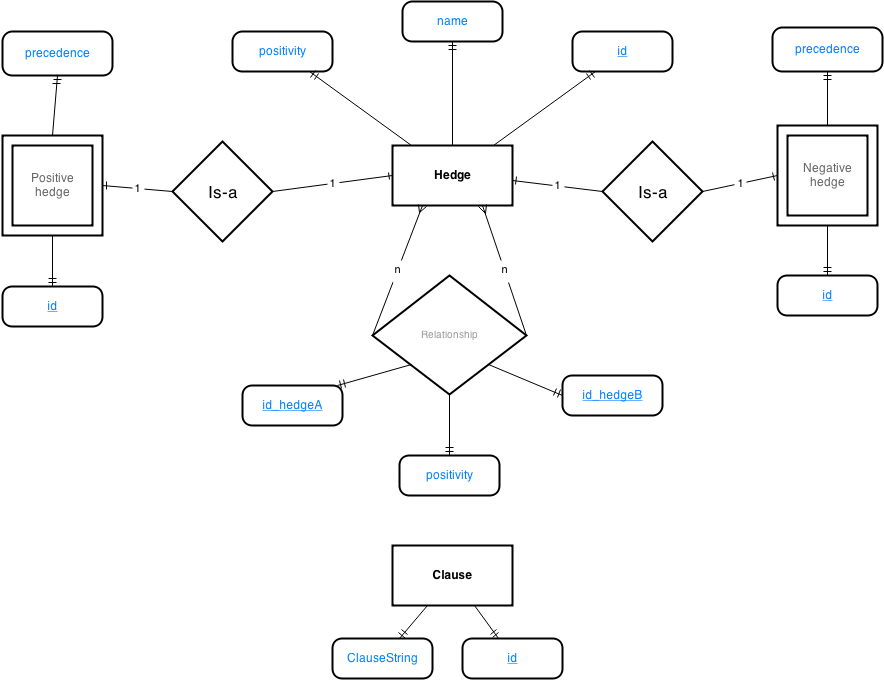
\includegraphics[scale=0.45]{ERDiagram}

\subsection{Table description}
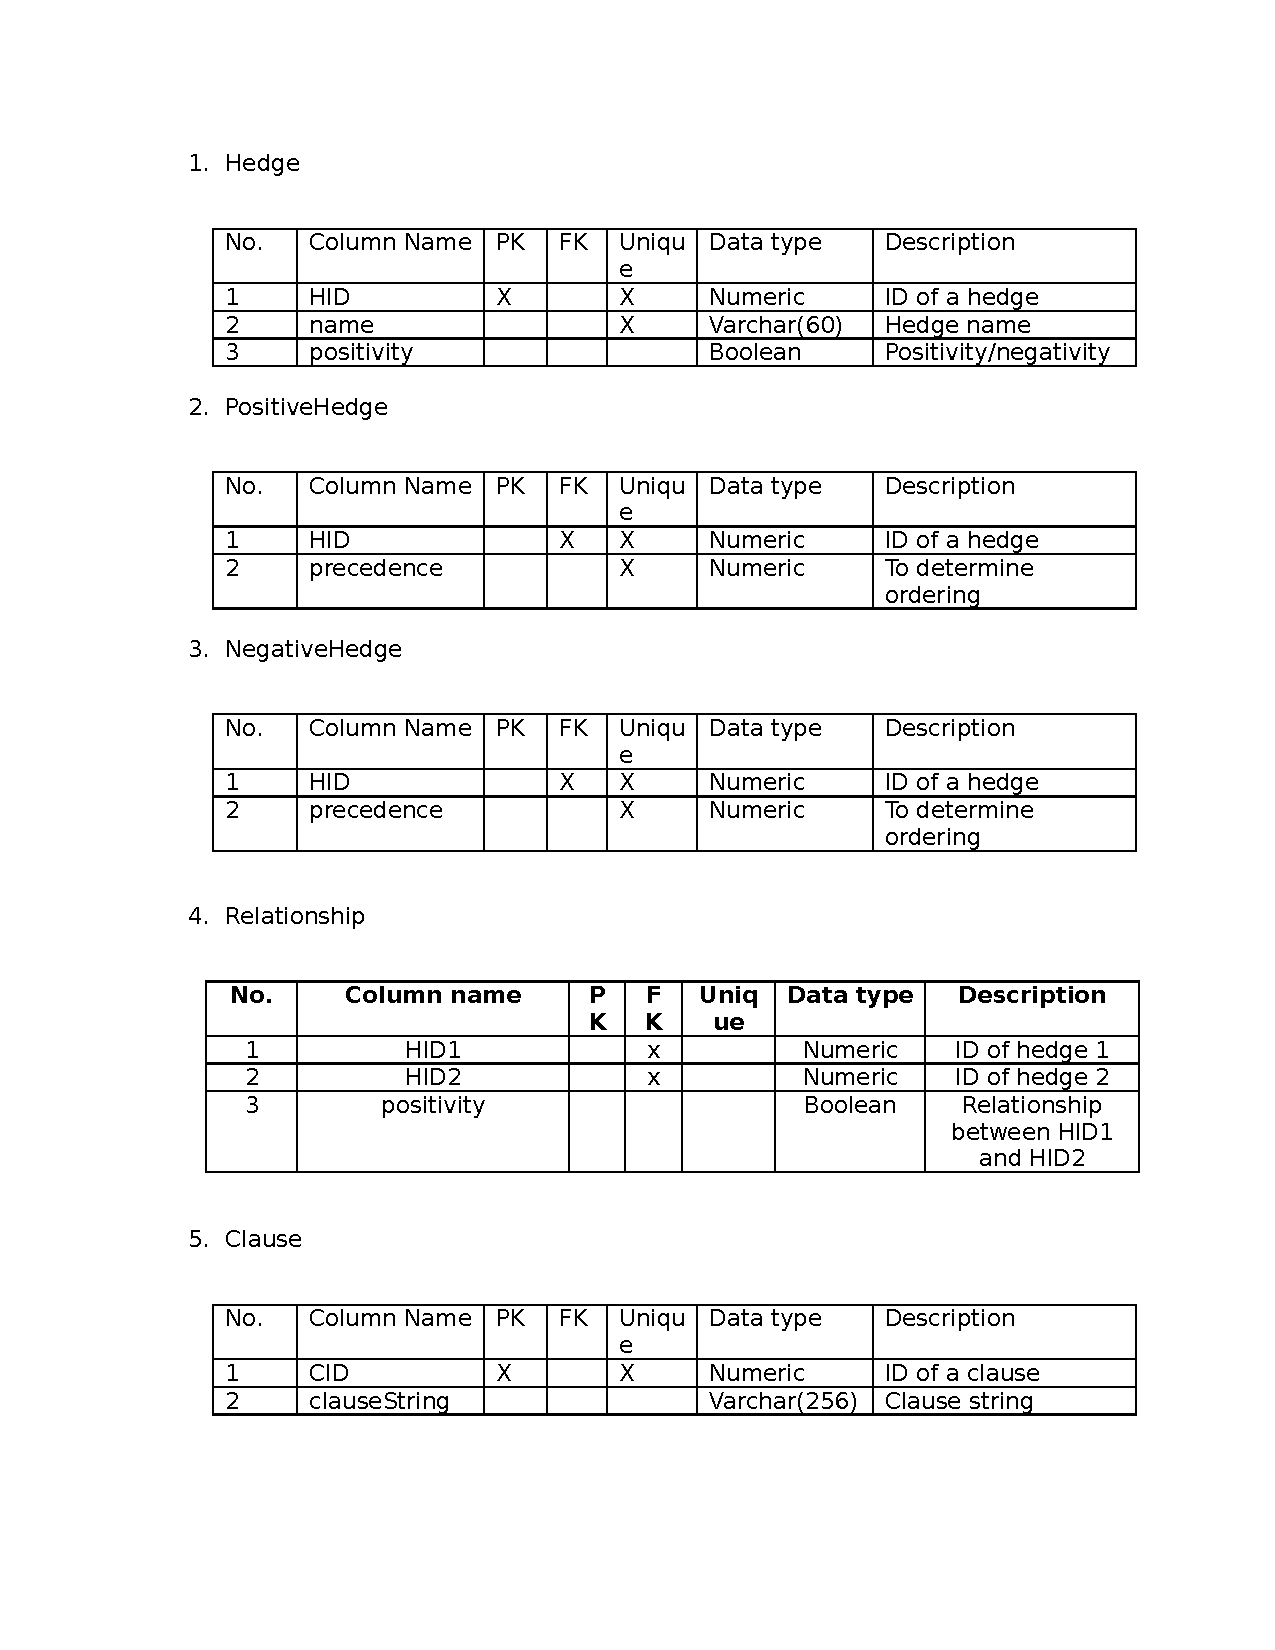
\includegraphics[clip=true, trim = 90 0 0 0, scale=0.8, page=1]{DataModel}

\section{Use cases}

\subsection{Use cases diagram}
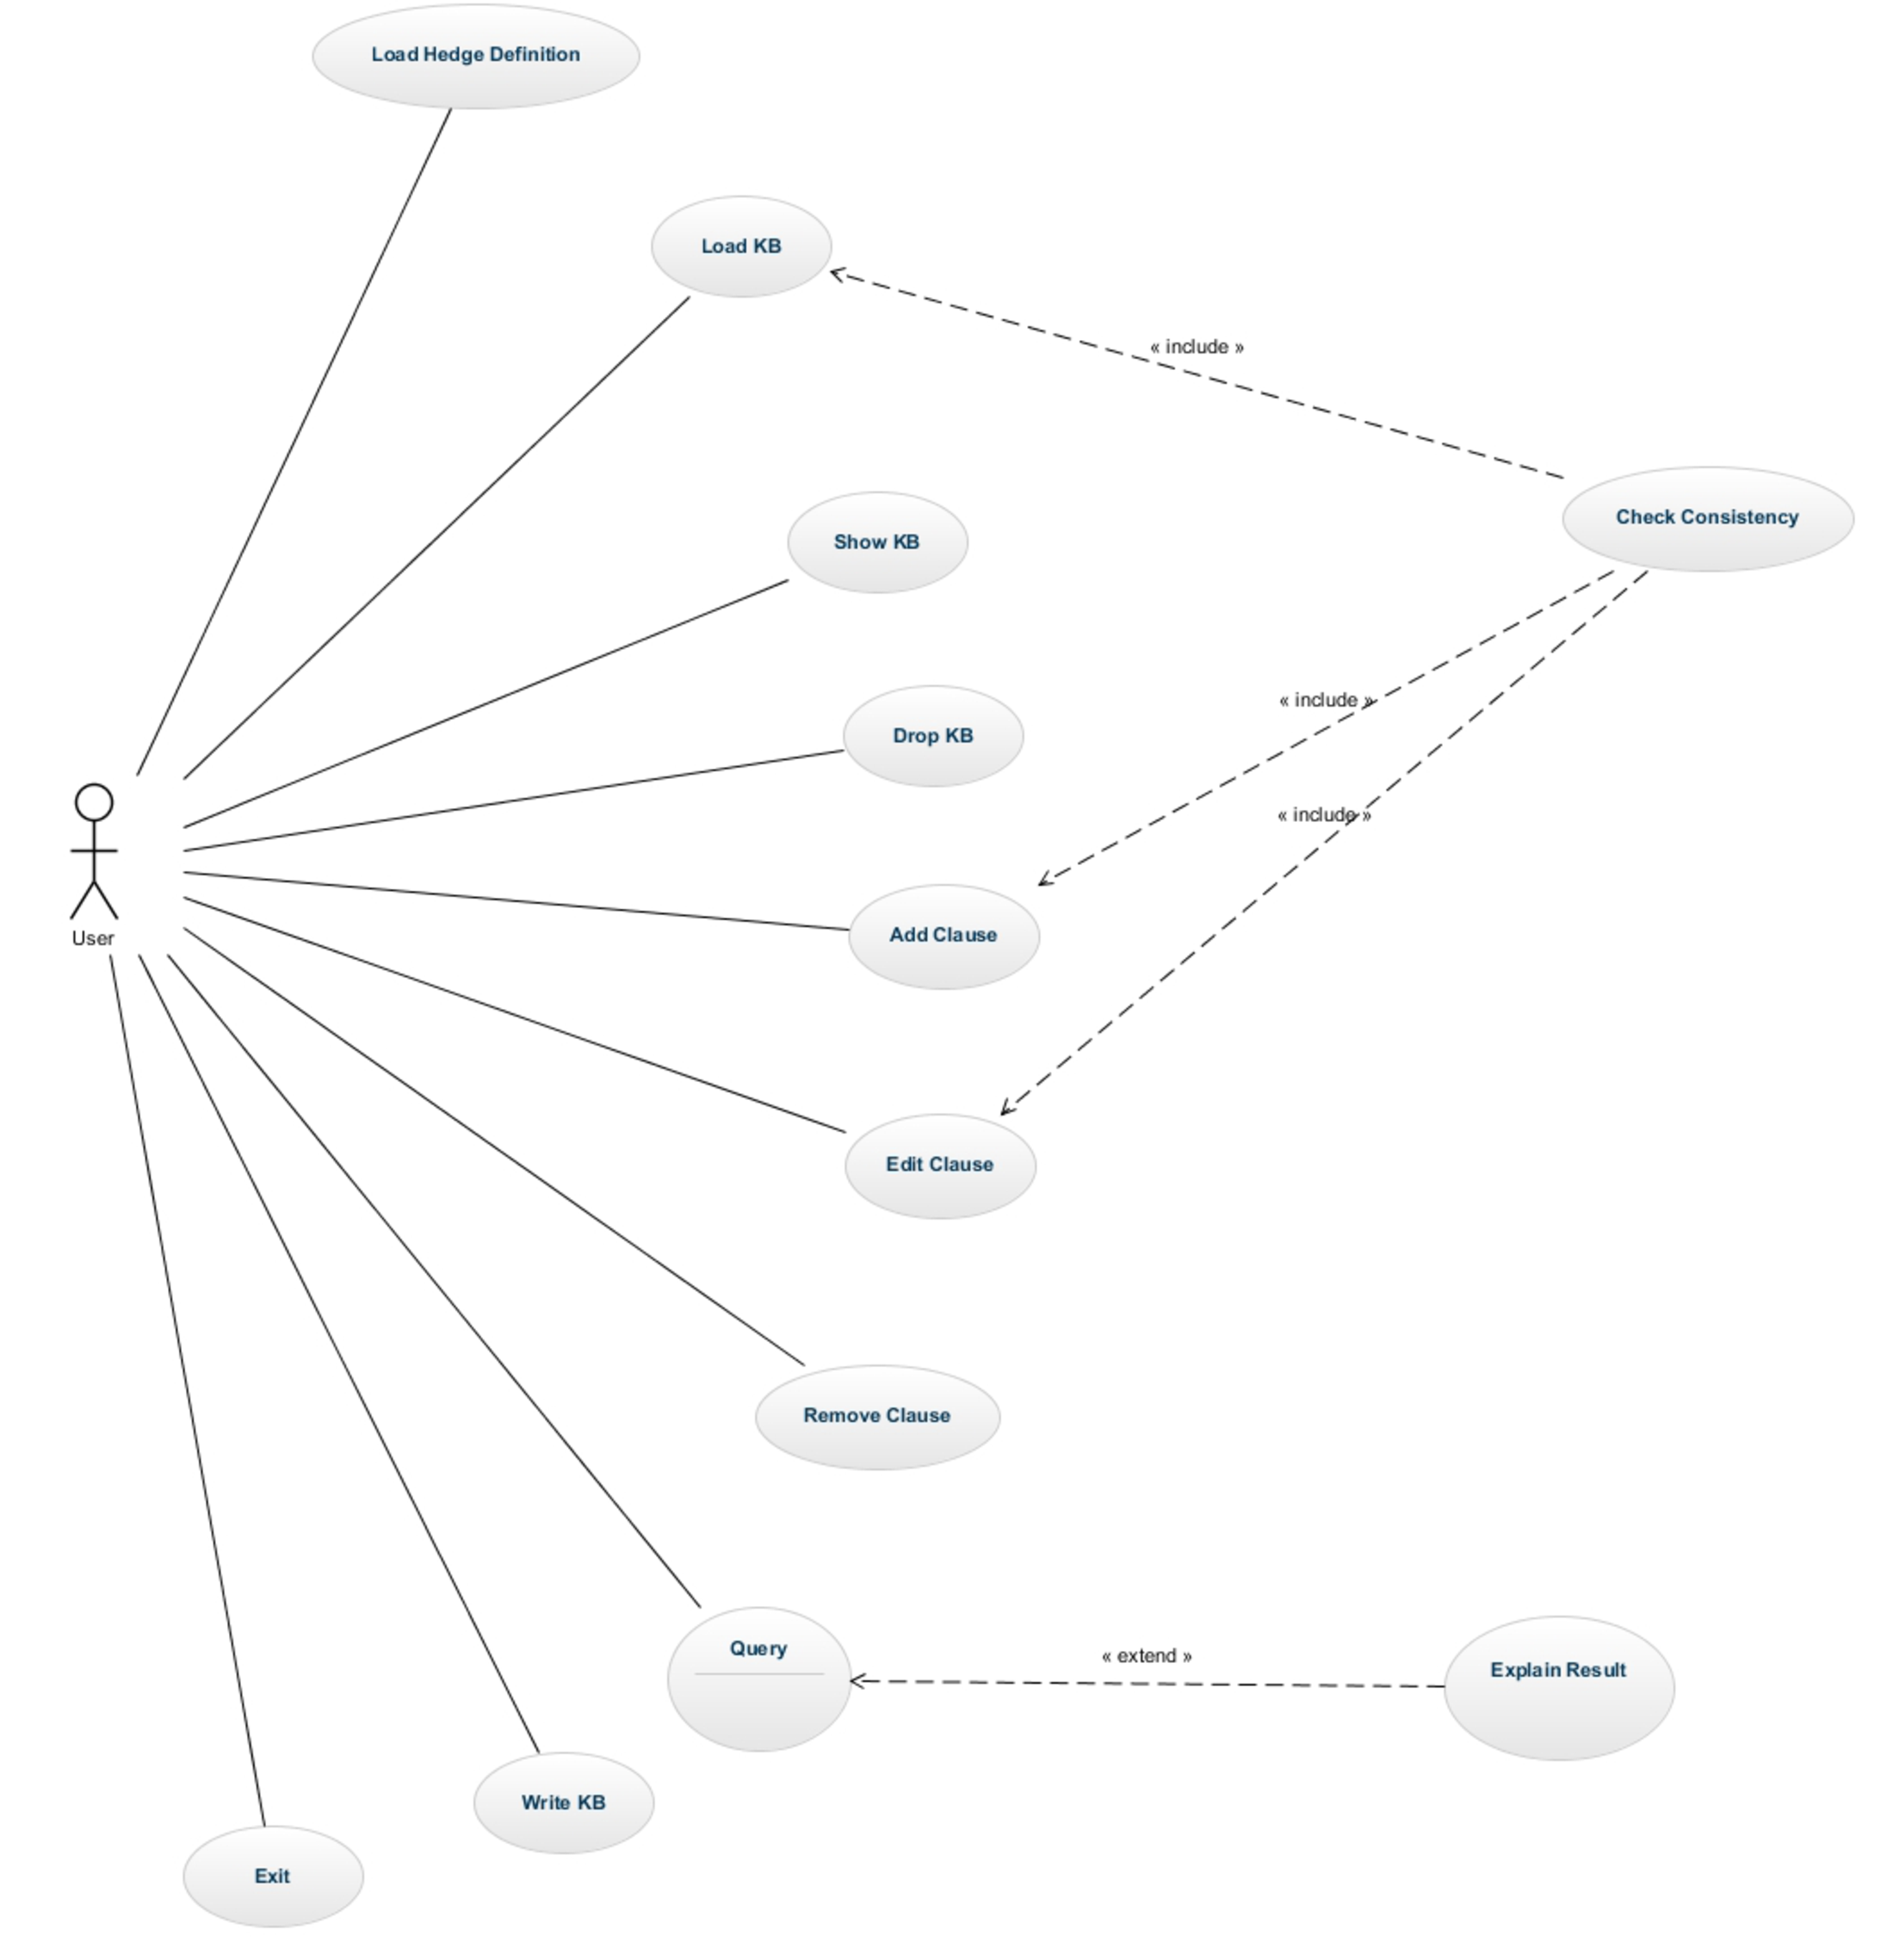
\includegraphics[scale=0.45]{UsecaseDiagram}

\subsection{Use cases specification}
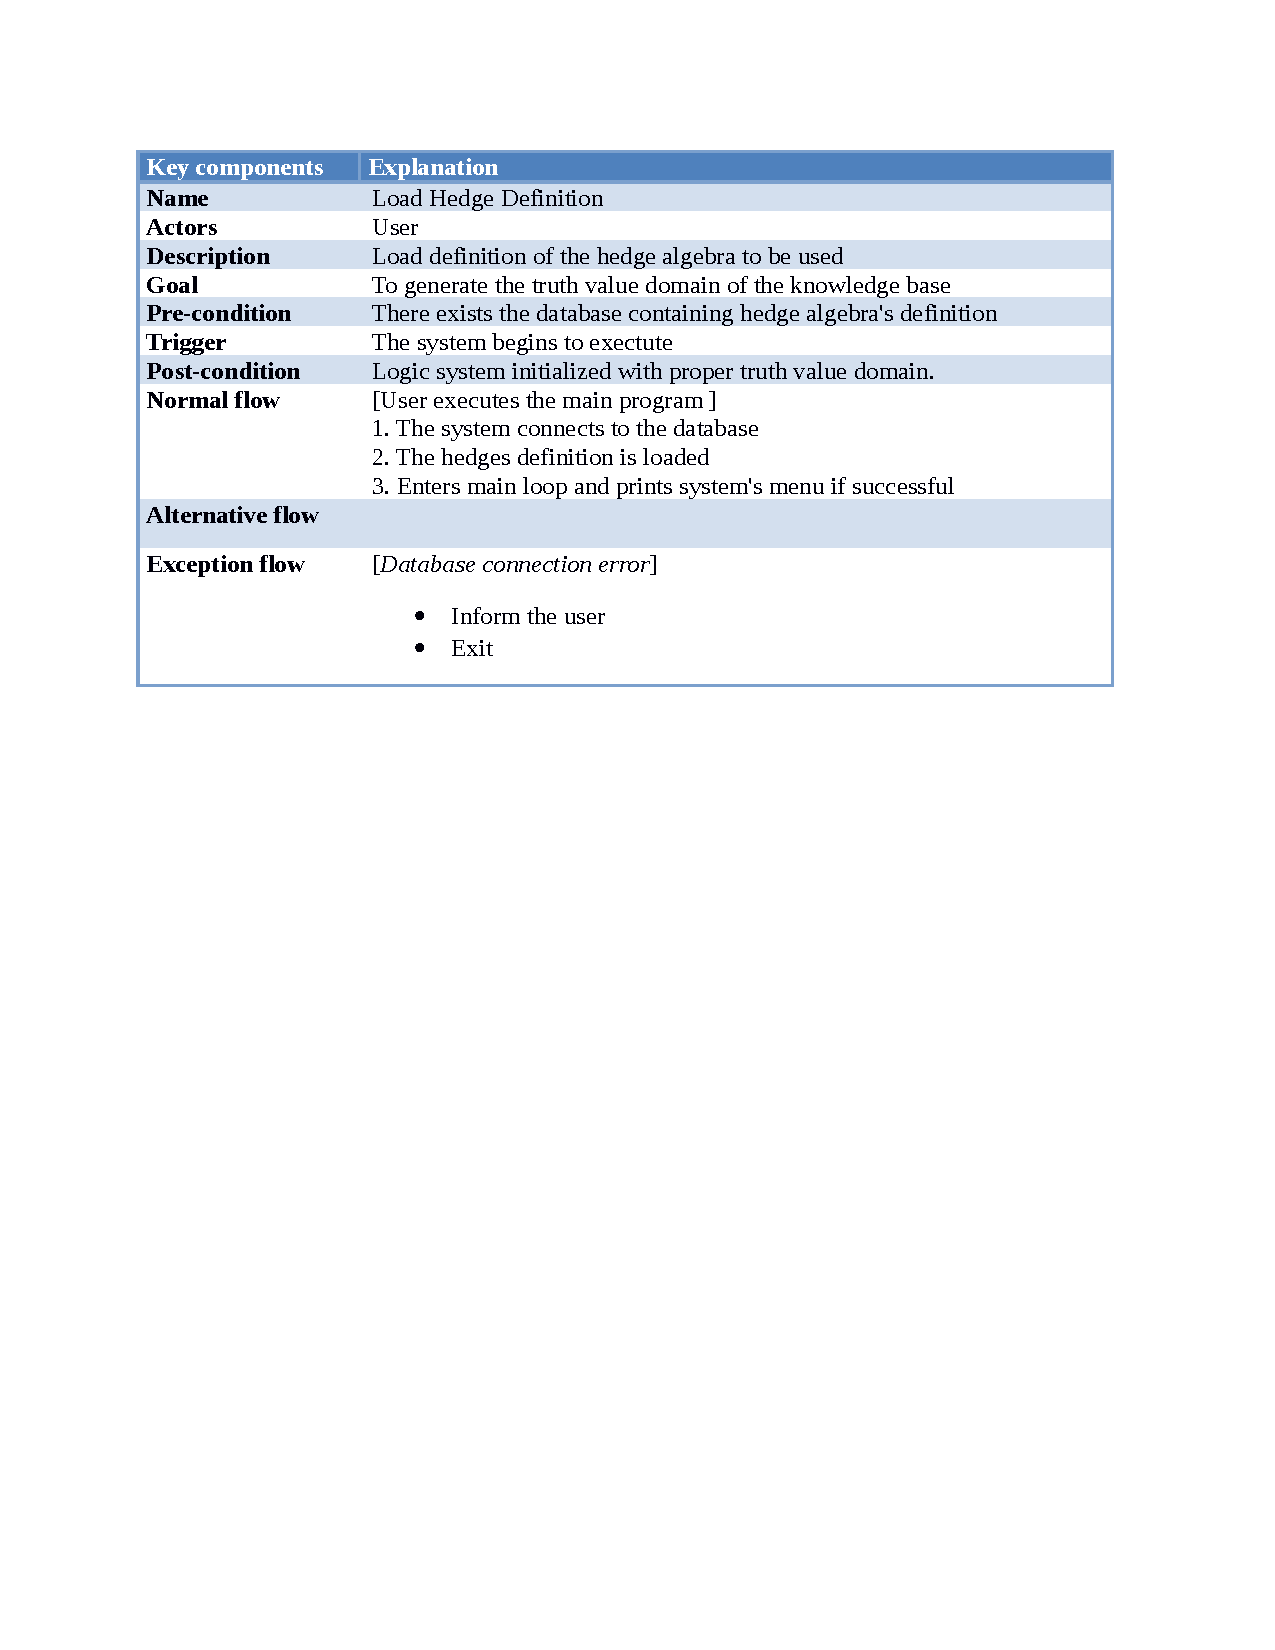
\includegraphics[clip=true, trim = 50 0 0 0, scale=0.8, page=1]{UCdesc}
\includegraphics[clip=true, trim = 50 0 0 0, scale=0.8, page=2]{UCdesc}
\includegraphics[clip=true, trim = 50 0 0 0, scale=0.8, page=3]{UCdesc}
\includegraphics[clip=true, trim = 50 0 0 0, scale=0.8, page=4]{UCdesc}
\includegraphics[clip=true, trim = 50 0 0 0, scale=0.8, page=5]{UCdesc}
\includegraphics[clip=true, trim = 50 0 0 0, scale=0.8, page=6]{UCdesc}
\includegraphics[clip=true, trim = 50 0 0 0, scale=0.8, page=7]{UCdesc}
\includegraphics[clip=true, trim = 50 0 0 0, scale=0.8, page=8]{UCdesc}
\includegraphics[clip=true, trim = 50 0 0 0, scale=0.8, page=9]{UCdesc}
\includegraphics[clip=true, trim = 50 0 0 0, scale=0.8, page=10]{UCdesc}
\includegraphics[clip=true, trim = 50 0 0 0, scale=0.8, page=11]{UCdesc}
\includegraphics[clip=true, trim = 50 0 0 0, scale=0.8, page=12]{UCdesc}



\section{Architectural design}

\subsection{Module HedgeClass}

\paragraph{}This module defines the Ha (short for Hedge algebra) typeclass, which is used as a basis for  actual hedge algebra. An instance Hedge of Ha (i.e. is the type for linguistic hedges) must define:

\begin{itemize}
\item A list of all linguistic hedges in the type Either a list of all
  positive hedges or a list of all negative hedges, or both list
\item  Either a positive relationship matrix, or a negative relationship
  matrix
\end{itemize}

\paragraph{}The Ha typeclass will accordingly generate:

\begin{itemize}
\item Operator <+> and <-> e.g. Very <+> Less = True means Very is
  positive w.r.t. Less, Less <-> Possibly = True means Less is
  negative w.r.t. 
\item Possibly Predicate positive and negative: Hedge ->
  Bool Comparing function compare': Hedge x Hedge -> LT | EQ | GT
\end{itemize}

\paragraph{}The HedgeClass module exports the typeclass Ha.

\subsection{Module HedgeTruth}


\paragraph{}This module defines the parametric type Truth. Given a type Hedge that is an instance of Ha, this parametric type will construct an actual linear symmetrical hedge algebra, with two generators: Tru being the positive one, Fals being the negative one. \\

\paragraph{}As an instance of the typeclass Ord, the compare function for Truth is also defined in this module, and is used as a basis for defining logical connectives for linguistic truth value.\\

\paragraph{}This module depends on the HedgeClass module, exports the type Truth, and the following functions:

\begin{itemize}
\item isHTrue, isHFalse: test whether if a truth value has True or
  False tendency 
\item andH, orH, notH: and, or and not counterparts for
  linguistic truth value 
\item operator (><): test whether if two linguistic
  truth value has opposite tendency or not
\end{itemize}


\subsection{Module ProsLogic}

\paragraph{}The representations for literals and clauses of the propositional language are defined here. It exports the Lit and CNF types and their type accessors/constructors. This module depends on the two modules HedgeClass and HedgeTruth.


\subsection{Module AlphaResolution}

\paragraph{}The implementation of Alpha Resolution method and its auxiliary functions are defined in this module. This resolution function takes a set of clauses and performs Alpha Resolution on it. The returned value is of the type Maybe (Truth hedge), where it can be Nothing if the resolution didn't entail the null clause, or Just <truth value> if it did.\\

\paragraph{}This module depends on HedgeClass, HedgeTruth and ProsLogic modules and exports the resolution procedure.

\subsection{Module HedgeGen}

\paragraph{}This module generate the Hedge type according to the description in the hedge database. Hedge will be an instance of Ha, and this module will export this type. This module depends on HedgeClass, and also import the libraries Template Haskell, HDBC and HDBC.SQLite3

\subsection{Module DatabaseIO}

\paragraph{}This module handles the connection and operations on the knowledge base DB. It depends on the libraries HDBC and HDBC.SQLite3, and exports the read, update and delete procedures.

\subsection{Module Main}

\paragraph{}This module is in charge of user interaction. The main loop is defined here.

\end {document}
